% Chapitre de découverte des services offerts
\chapter{Découvrir les différents services}
%\addcontentsline{toc}{chapter}{Découvrir les différents services}

Le portail est le centre névralgique de l'environnement de la Boîte. 
Au début il est pour ainsi dire vide sauf la présence dans l'espace, en haut, d'une barre avec plusieurs onglets~:
\begin{figure}
	\centering
	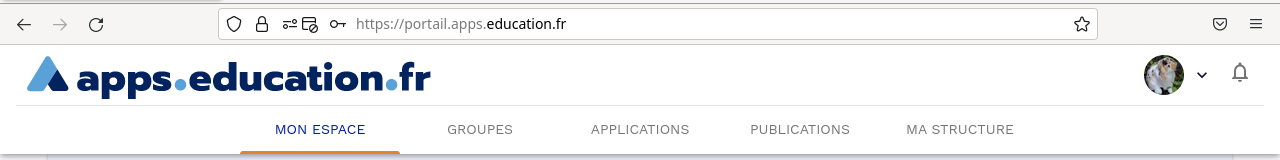
\includegraphics[width=\linewidth]{./Captures/portail.barre.haute.png}
%	\caption{}
\end{figure}
Deux onglets seront intéressants dans les premiers temps, celui des groupes et celui des applications puisque leur rôle est d'ajouter de nouvelles vignettes au sein de l'accueil (onglet de gauche).

Une fois que vous aurez ajouté les applications ou les groupes, votre portail pourra évoluer et par exemple ressembler à celui-ci~:
\begin{figure}
	\centering
	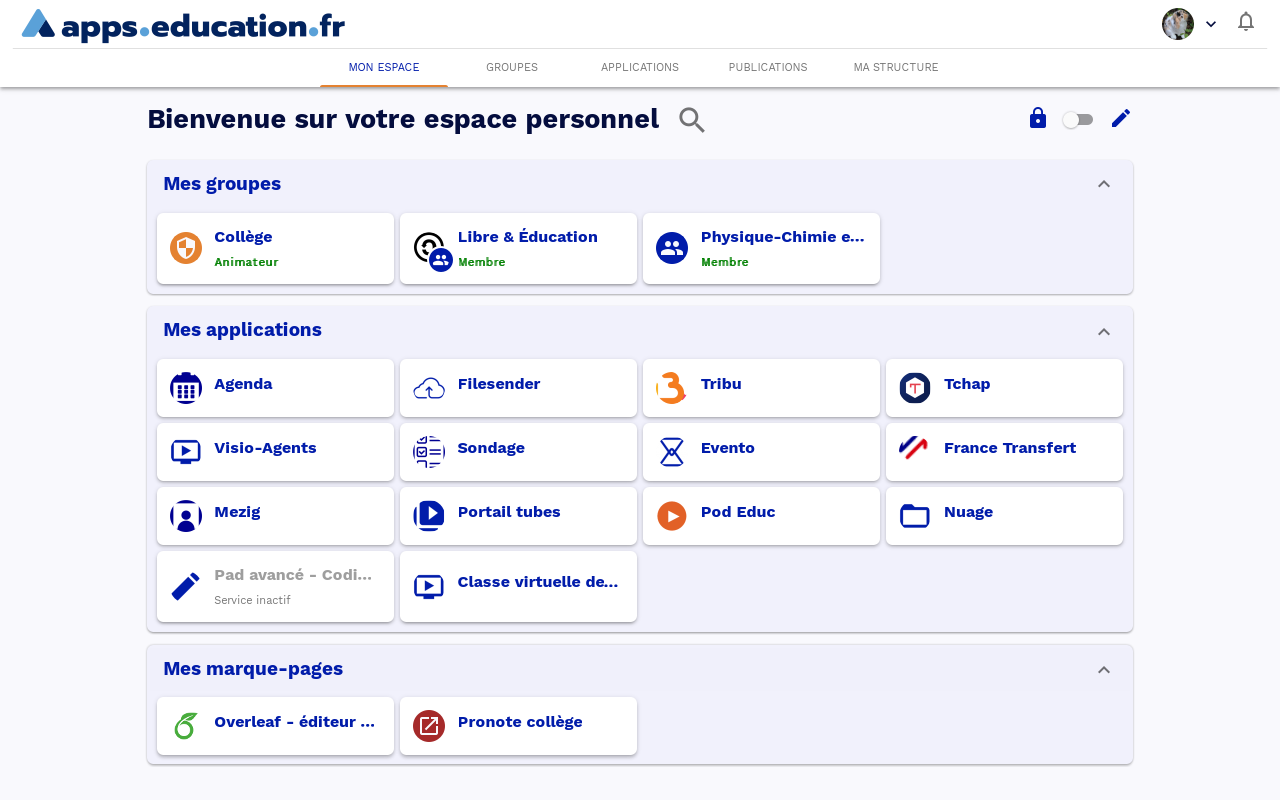
\includegraphics[width=\linewidth]{./Captures/portail.accueil.png}
%	\caption{}
\end{figure}

